\documentclass[12pt,letterpaper]{article}

\usepackage[margin=0.75in]{geometry}
\usepackage{amsmath,amssymb,amsthm}
\usepackage{enumitem}
\usepackage{tikz}

\pagestyle{plain}
\setlength{\parindent}{0pt}
\setlength{\parskip}{0.5em}
\setlength{\emergencystretch}{2em}

\theoremstyle{definition}
\newtheorem{theorem}{Theorem}[section]
\newtheorem{lemma}[theorem]{Lemma}
\newtheorem{corollary}[theorem]{Corollary}
\newtheorem{proposition}[theorem]{Proposition}
\newtheorem{definition}[theorem]{Definition}
\newtheorem{example}[theorem]{Example}
\newtheorem*{remark}{Remark}

\DeclareMathOperator{\arcsec}{arcsec}
\DeclareMathOperator{\arccot}{arccot}
\DeclareMathOperator{\arccsc}{arccsc}

\begin{document}

\begin{center}
  {\large\bfseries MATH 15200: Calculus II}\\
  {\large\bfseries Lecture Notes: Inverse Functions, Inverse Trigonometric
    Functions, and Integration by Parts}\\[0.3em]
  Salas, Hille, and Etgen, \S\S7.1, 7.7, and 8.2
\end{center}

\vspace{0.25em}
\hrule
\vspace{0.8em}

%----------------------------------------------------------------------------
\section{Inverse functions}

\begin{definition}
  A function $f$ is \emph{one-to-one} if $f(x_1)=f(x_2)$ implies $x_1=x_2$;
  that is, $f$ never takes the same value at two different points. If $f$ is
  one-to-one with domain $D$ and range $R$, its \emph{inverse} is the function
  $f^{-1}\colon R\to D$ defined by
  \[
    f^{-1}(y)=\text{the unique $x\in D$ with $f(x)=y$}.
  \]
\end{definition}

The following facts come straight from the definition.
\begin{itemize}[itemsep=0.2em]
  \item $f^{-1}\bigl(f(x)\bigr)=x$ for every $x\in D$, and
    $f\bigl(f^{-1}(y)\bigr)=y$ for every $y\in R$.
  \item The domain of $f^{-1}$ is the range of $f$, and the range of $f^{-1}$
    is the domain of $f$.
  \item $(a,b)$ lies on the graph of $f$ if and only if $(b,a)$ lies on the
    graph of $f^{-1}$. So the graph of $f^{-1}$ is the reflection of the graph
    of $f$ across the line $y=x$.
  \item Warning: $f^{-1}(x)$ does not mean $1/f(x)$.
\end{itemize}

\begin{example}
  \begin{enumerate}[label=(\alph*)]
    \item $f(x)=2x+3$ is one-to-one on $\mathbb{R}$. To find $f^{-1}$, solve
      $y=2x+3$ for $x$ to get $x=\frac{y-3}{2}$. So
      $f^{-1}(x)=\frac{x-3}{2}$.
    \item $f(x)=x^2$ is not one-to-one on $\mathbb{R}$, since $f(-1)=f(1)$.
      It is one-to-one on $[0,\infty)$, and the inverse of this restricted
      function is $\sqrt{x}$. We will do the same thing with the
      trigonometric functions in Section~\ref{sec:inverse-trig}: restrict the
      domain to make the function one-to-one, then invert.
  \end{enumerate}
\end{example}

\textbf{Monotonic functions are one-to-one.}

\begin{theorem}
  If $f$ is strictly increasing or strictly decreasing on its domain, then $f$
  is one-to-one.
\end{theorem}

\begin{proof}
  Let $x_1\neq x_2$, say $x_1<x_2$. Then either $f(x_1)<f(x_2)$ or
  $f(x_1)>f(x_2)$; in either case $f(x_1)\neq f(x_2)$.
\end{proof}

Recall from the Mean Value Theorem that if $f'>0$ on an interval, then $f$ is
strictly increasing there, and if $f'<0$, then $f$ is strictly decreasing.
This stays true if $f'$ vanishes at finitely many points (apply the MVT on each
piece). For instance, $x^3$ is strictly increasing on $\mathbb{R}$ even though
its derivative is $0$ at $0$.

\begin{remark}
  Conversely, a continuous function that is one-to-one on an interval must be
  strictly increasing or strictly decreasing there (this follows from the
  Intermediate Value Theorem). We won't need this: in practice, we check that a
  function is one-to-one by checking the sign of its derivative.
\end{remark}

\begin{example}\label{ex:cubic}
  Let $f(x)=x^3+x$. Since $f'(x)=3x^2+1>0$, $f$ is strictly increasing, and so
  one-to-one, on $\mathbb{R}$. Its range is all of $\mathbb{R}$: $f$ is
  continuous and $f(x)\to\pm\infty$ as $x\to\pm\infty$, so by the IVT it takes
  every real value. So $f^{-1}$ is defined on all of $\mathbb{R}$.

  However, solving $y=x^3+x$ for $x$ requires the cubic formula, so there is
  no convenient formula for $f^{-1}$. We can still read off some values:
  $f(0)=0$, $f(1)=2$, and $f(2)=10$, so $f^{-1}(0)=0$, $f^{-1}(2)=1$, and
  $f^{-1}(10)=2$.

  \emph{Question:} What is the slope of the graph of $f^{-1}$ at $x=2$? We
  will answer this in Example~\ref{ex:cubic-derivative}, without ever finding
  a formula for $f^{-1}$.
\end{example}

\textbf{Exponential and logarithm.} Recall that $\ln$ is strictly increasing
on $(0,\infty)$, since its derivative is $1/x>0$, that its range is
$\mathbb{R}$, and that its inverse is the exponential function $e^x$. So
$e^{\ln x}=x$ for $x>0$ and $\ln(e^x)=x$ for all $x$, and the graphs of $e^x$
and $\ln x$ are reflections of each other across $y=x$.

\begin{center}
  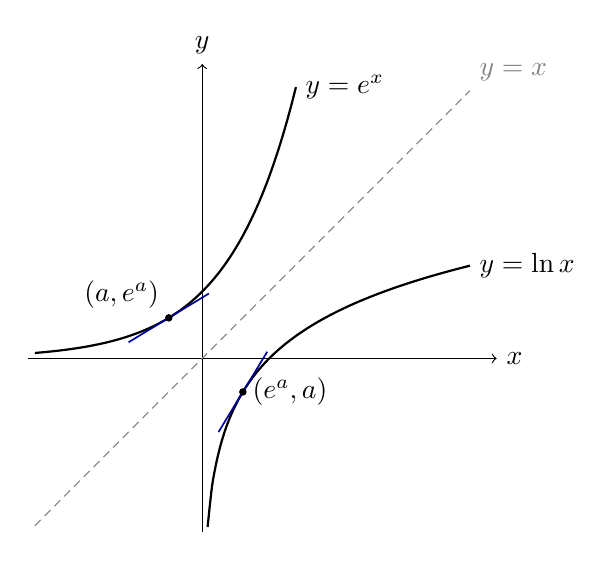
\begin{tikzpicture}[scale=0.85]
    \pgfmathsetmacro{\pa}{-0.5}
    \pgfmathsetmacro{\pb}{exp(\pa)}
    \draw[->] (-2.6,0) -- (4.4,0) node[right] {$x$};
    \draw[->] (0,-2.6) -- (0,4.4) node[above] {$y$};
    \draw[densely dashed, gray] (-2.5,-2.5) -- (4,4);
    \node[gray, above right] at (4,4) {$y=x$};
    \draw[thick, domain=-2.5:1.4, samples=60, smooth]
      plot (\x, {exp(\x)});
    \node[right] at (1.4,{exp(1.4)}) {$y=e^x$};
    \draw[thick, domain=0.08:4, samples=60, smooth]
      plot (\x, {ln(\x)});
    \node[right] at (4,{ln(4)}) {$y=\ln x$};
    % Tangent lines at (a, e^a) and at its reflection (e^a, a).
    \draw[blue!60!black, semithick]
      ({\pa-0.6},{\pb-0.6*\pb}) -- ({\pa+0.6},{\pb+0.6*\pb});
    \draw[blue!60!black, semithick]
      ({\pb-0.6*\pb},{\pa-0.6}) -- ({\pb+0.6*\pb},{\pa+0.6});
    \fill (\pa,\pb) circle[radius=1.6pt];
    \node[above left] at (\pa,\pb) {$(a,e^a)$};
    \fill (\pb,\pa) circle[radius=1.6pt];
    \node[right] at (\pb,\pa) {$(e^a,a)$};
  \end{tikzpicture}
\end{center}

The tangent lines at $(a,e^a)$ and $(e^a,a)$ are also reflections of each
other. Reflecting across $y=x$ swaps rise and run, so their slopes, $e^a$ and
$1/e^a$, are reciprocals. This is the idea behind the next section.

%----------------------------------------------------------------------------
\section{Derivatives of inverse functions}

\textbf{The formula, if we assume the derivative exists.} Suppose $f$ is
one-to-one and differentiable, and suppose we already knew that $f^{-1}$ is
differentiable. Differentiating both sides of $f\bigl(f^{-1}(x)\bigr)=x$ with
the chain rule gives
\[
  f'\bigl(f^{-1}(x)\bigr)\cdot(f^{-1})'(x)=1,
  \qquad\text{so}\qquad
  (f^{-1})'(x)=\frac{1}{f'\bigl(f^{-1}(x)\bigr)}.
\]
This is the correct formula, and this computation is the easiest way to
remember it. But it is not a proof: it \emph{assumes} that $f^{-1}$ is
differentiable, and that is the main thing to prove.

\begin{theorem}[Derivative of an inverse]\label{thm:inverse-derivative}
  Let $f$ be differentiable and strictly monotonic on an open interval $I$,
  let $J=f(I)$, and let $g=f^{-1}\colon J\to I$. Let $a\in I$ and $b=f(a)$. If
  $f'(a)\neq0$, then $g$ is differentiable at $b$, and
  \[
    g'(b)=\frac{1}{f'(a)}=\frac{1}{f'\bigl(g(b)\bigr)}.
  \]
\end{theorem}

The proof rests on the continuity of $g$, which we prove first.

\begin{lemma}\label{lem:inverse-continuous}
  Let $f$ be continuous and strictly increasing on an open interval $I$, let
  $J=f(I)$, and let $g=f^{-1}\colon J\to I$.
  \begin{enumerate}[label=(\alph*)]
    \item $g$ is strictly increasing.
    \item Every $b\in J$ is an interior point of $J$; that is, $J$ contains an
      open interval around $b$.
    \item $g$ is continuous on $J$.
  \end{enumerate}
\end{lemma}

\begin{proof}
  (a) Suppose $y_1<y_2$ in $J$, but $g(y_1)\geq g(y_2)$. Applying the
  increasing function $f$ gives $y_1\geq y_2$, a contradiction.

  (b) Let $a=g(b)$. Since $I$ is open, there is an $h>0$ with
  $[a-h,a+h]\subseteq I$. Then $f(a-h)<b<f(a+h)$, and by the IVT, $f$ takes
  every value between $f(a-h)$ and $f(a+h)$ on $[a-h,a+h]$. So the open
  interval $\bigl(f(a-h),f(a+h)\bigr)$ lies in $J$ and contains $b$.

  (c) Let $b\in J$, let $a=g(b)$, and let $\varepsilon>0$. Shrinking
  $\varepsilon$ only makes what we must prove stronger, so we may assume that
  $[a-\varepsilon,a+\varepsilon]\subseteq I$. Then
  $f(a-\varepsilon)<b<f(a+\varepsilon)$, so
  \[
    \delta=\min\bigl\{\,b-f(a-\varepsilon),\ f(a+\varepsilon)-b\,\bigr\}>0.
  \]
  If $y\in J$ and $|y-b|<\delta$, then $f(a-\varepsilon)<y<f(a+\varepsilon)$.
  Applying $g$, which is increasing by (a), gives
  $a-\varepsilon<g(y)<a+\varepsilon$; that is, $|g(y)-g(b)|<\varepsilon$.
\end{proof}

\begin{proof}[Proof of Theorem~\ref{thm:inverse-derivative}]
  We treat the case where $f$ is increasing; the decreasing case is the same
  with the inequalities reversed. Since $f$ is differentiable, it is
  continuous, so Lemma~\ref{lem:inverse-continuous} applies. By part~(b), $g$
  is defined on an open interval around $b$, so it makes sense to ask whether
  $g$ is differentiable at $b$.

  For $x\in I$ with $x\neq a$, let
  \[
    Q(x)=\frac{f(x)-f(a)}{x-a}.
  \]
  Then $Q(x)\to f'(a)$ as $x\to a$, and $Q(x)\neq0$ because $f$ is one-to-one.
  Now let $y\in J$ with $y\neq b$, and let $x=g(y)$. Then $f(x)=y$, and
  $x\neq a$ because $g$ is one-to-one. So
  \[
    \frac{g(y)-g(b)}{y-b}=\frac{x-a}{f(x)-f(a)}=\frac{1}{Q(x)}
      =\frac{1}{Q\bigl(g(y)\bigr)}.
  \]

  \emph{Claim:} $Q\bigl(g(y)\bigr)\to f'(a)$ as $y\to b$. Let
  $\varepsilon>0$. Choose $\eta>0$ such that $|Q(x)-f'(a)|<\varepsilon$
  whenever $0<|x-a|<\eta$. Since $g$ is continuous at $b$
  (Lemma~\ref{lem:inverse-continuous}(c)), we can choose $\delta>0$ such that
  $|g(y)-a|<\eta$ whenever $y\in J$ and $|y-b|<\delta$. If
  $0<|y-b|<\delta$, then $g(y)\neq a$, so $0<|g(y)-a|<\eta$, and hence
  $\bigl|Q\bigl(g(y)\bigr)-f'(a)\bigr|<\varepsilon$.

  Finally, since $f'(a)\neq0$, the quotient rule for limits gives
  \[
    \lim_{y\to b}\frac{g(y)-g(b)}{y-b}
      =\lim_{y\to b}\frac{1}{Q\bigl(g(y)\bigr)}=\frac{1}{f'(a)}.
    \qedhere
  \]
\end{proof}

\begin{remark}
  The heart of the proof is that $x=g(y)\to a$ as $y\to b$, which is the
  continuity of $g$. The hypothesis $f'(a)\neq0$ is used only in the last
  step.
\end{remark}

\begin{corollary}\label{cor:inverse-derivative}
  If $f$ is differentiable on an open interval $I$ with $f'>0$ on $I$ (or
  $f'<0$ on $I$), then $f^{-1}$ is differentiable on $J=f(I)$, and
  \[
    (f^{-1})'(x)=\frac{1}{f'\bigl(f^{-1}(x)\bigr)}
    \qquad\text{for all } x\in J.
  \]
\end{corollary}

\begin{remark}
  The hypothesis $f'(a)\neq0$ cannot be dropped. If $f'(a)=0$ and $g$ were
  differentiable at $b$, then the chain rule applied to $f\bigl(g(y)\bigr)=y$
  at $y=b$ would give $f'(a)\,g'(b)=1$, that is, $0=1$. So in this case $g$ is
  \emph{not} differentiable at $b$. For example, $f(x)=x^3$ is strictly
  increasing on $\mathbb{R}$ with $f'(0)=0$, and its inverse $\sqrt[3]{x}$ is
  not differentiable at $0$. Its graph has a vertical tangent there, which is
  the reflection of the horizontal tangent of $x^3$ at the origin.
\end{remark}

\begin{example}\label{ex:cubic-derivative}
  Return to $f(x)=x^3+x$ from Example~\ref{ex:cubic}. Since
  $f'(x)=3x^2+1>0$, Corollary~\ref{cor:inverse-derivative} applies. To find
  $(f^{-1})'(2)$ we need $f^{-1}(2)$, which is $1$ because $f(1)=2$. So
  \[
    (f^{-1})'(2)=\frac{1}{f'(1)}=\frac14,
  \]
  and the tangent line to the graph of $f^{-1}$ at $(2,1)$ is
  $y=1+\frac14(x-2)$. Similarly, $f(2)=10$ gives
  $(f^{-1})'(10)=1/f'(2)=1/13$.

  The key step is always the same: to evaluate $(f^{-1})'$ at $b$, first find
  the $a$ with $f(a)=b$.
\end{example}

\begin{example}
  Since $\ln$ is differentiable on $(0,\infty)$ with derivative $1/x>0$,
  Corollary~\ref{cor:inverse-derivative} shows that $e^x$ is differentiable
  on $\mathbb{R}$, and
  \[
    \frac{d}{dx}e^x=\frac{1}{\ln'(e^x)}=\frac{1}{1/e^x}=e^x.
  \]
  In particular, the corollary guarantees that $e^x$ is differentiable, which
  is exactly what is needed to justify differentiating $\ln(e^x)=x$ with the
  chain rule.
\end{example}

\begin{example}
  Let $f(x)=x^2$ on $(0,\infty)$, where $f'(x)=2x>0$. Its inverse is
  $\sqrt{x}$, so
  \[
    \frac{d}{dx}\sqrt{x}=\frac{1}{f'(\sqrt{x})}=\frac{1}{2\sqrt{x}},
  \]
  as expected. In the same way, for an integer $n\geq2$, the inverse of $x^n$
  on $(0,\infty)$ is $x^{1/n}$, and
  \[
    \frac{d}{dx}x^{1/n}=\frac{1}{n\bigl(x^{1/n}\bigr)^{n-1}}
      =\frac1n\,x^{\frac1n-1}.
  \]
\end{example}

\begin{example}
  Let $F(x)=\displaystyle\int_2^x\sqrt{t^4+9}\,dt$. Find $(F^{-1})'(0)$.

  By the Fundamental Theorem of Calculus, $F'(x)=\sqrt{x^4+9}>0$, so $F$ is
  strictly increasing, and so one-to-one, on $\mathbb{R}$. Since
  $F(2)=\int_2^2\sqrt{t^4+9}\,dt=0$, we have $F^{-1}(0)=2$. So
  \[
    (F^{-1})'(0)=\frac{1}{F'(2)}=\frac{1}{\sqrt{25}}=\frac15.
  \]
\end{example}

%----------------------------------------------------------------------------
\section{Inverse trigonometric functions}\label{sec:inverse-trig}

The trigonometric functions are periodic, so none of them is one-to-one. To
invert one, we restrict it to a set where it is one-to-one and invert the
restriction. The choice of set is a convention; we use the same choices as
Salas.

\subsection{Arcsine}

Since $\sin'=\cos>0$ on $(-\frac\pi2,\frac\pi2)$, $\sin$ is strictly
increasing on $[-\frac\pi2,\frac\pi2]$, and it goes from
$\sin(-\frac\pi2)=-1$ to $\sin\frac\pi2=1$. So on this interval it takes each
value in $[-1,1]$ exactly once: at least once by the IVT, and at most once
because it is increasing.

\begin{definition}
  For $-1\leq x\leq1$, $\arcsin x$ is the unique number $\theta$ in
  $[-\frac\pi2,\frac\pi2]$ with $\sin\theta=x$.
\end{definition}

In words: $\arcsin x$ is the angle between $-\frac\pi2$ and $\frac\pi2$ whose
sine is $x$.
\begin{itemize}[itemsep=0.2em]
  \item The domain of $\arcsin$ is $[-1,1]$, and its range is
    $[-\frac\pi2,\frac\pi2]$.
  \item $\sin(\arcsin x)=x$ for every $x\in[-1,1]$.
  \item $\arcsin(\sin\theta)=\theta$ \emph{only} for
    $\theta\in[-\frac\pi2,\frac\pi2]$.
  \item $\arcsin$ is increasing and odd: $\arcsin(-x)=-\arcsin x$.
  \item Notation: $\arcsin x$ is also written $\sin^{-1}x$. This does not
    mean $(\sin x)^{-1}=\csc x$, even though $\sin^2x$ means $(\sin x)^2$.
\end{itemize}

\begin{center}
  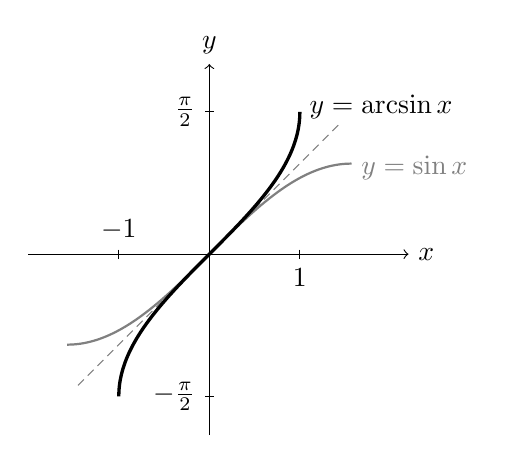
\begin{tikzpicture}[scale=1.15]
    \draw[->] (-2,0) -- (2.2,0) node[right] {$x$};
    \draw[->] (0,-2) -- (0,2.1) node[above] {$y$};
    \draw[densely dashed, gray] (-1.45,-1.45) -- (1.45,1.45);
    \draw[thick, gray, domain=-1.5708:1.5708, samples=50, smooth]
      plot (\x, {sin(\x r)});
    \draw[very thick, variable=\t, domain=-1.5708:1.5708, samples=50, smooth]
      plot ({sin(\t r)}, \t);
    \foreach \v in {-1,1} \draw (\v,0.05) -- (\v,-0.05);
    \node[below] at (1,-0.05) {$1$};
    \node[above] at (-1,0.05) {$-1$};
    \draw (0.05,1.5708) -- (-0.05,1.5708) node[left] {$\frac\pi2$};
    \draw (0.05,-1.5708) -- (-0.05,-1.5708) node[left] {$-\frac\pi2$};
    \node[right] at (1,1.62) {$y=\arcsin x$};
    \node[right, gray] at (1.57,0.95) {$y=\sin x$};
  \end{tikzpicture}
\end{center}

\begin{example}
  \begin{enumerate}[label=(\alph*)]
    \item $\arcsin\frac12=\frac\pi6$, $\arcsin\bigl(-\frac{\sqrt3}{2}\bigr)
      =-\frac\pi3$, $\arcsin1=\frac\pi2$, and $\arcsin0=0$.
    \item $\arcsin\bigl(\sin\frac{5\pi}{6}\bigr)=\arcsin\frac12=\frac\pi6$,
      \emph{not} $\frac{5\pi}{6}$, because $\frac{5\pi}{6}$ is not in
      $[-\frac\pi2,\frac\pi2]$.
    \item $\arcsin(\sin4)=\pi-4$. Indeed, $\sin(\pi-4)=\sin4$, and since
      $\pi<4<\frac{3\pi}{2}$, the number $\pi-4$ lies in
      $(-\frac\pi2,0)$.
  \end{enumerate}
\end{example}

\begin{theorem}\label{thm:arcsin-derivative}
  $\arcsin$ is differentiable on $(-1,1)$, and
  \[
    \frac{d}{dx}\arcsin x=\frac{1}{\sqrt{1-x^2}}
    \qquad(-1<x<1).
  \]
\end{theorem}

\begin{proof}
  Apply Corollary~\ref{cor:inverse-derivative} to $f=\sin$ on the open
  interval $I=(-\frac\pi2,\frac\pi2)$, where $f'(\theta)=\cos\theta>0$; here
  $J=(-1,1)$. For $-1<x<1$, let $\theta=\arcsin x$. Then
  \[
    \frac{d}{dx}\arcsin x=\frac{1}{\cos\theta}.
  \]
  Since $\theta\in(-\frac\pi2,\frac\pi2)$, we have $\cos\theta>0$, so
  $\cos\theta=\sqrt{1-\sin^2\theta}=\sqrt{1-x^2}$.
\end{proof}

\begin{remark}
  For $0<x<1$ there is a picture: $\theta=\arcsin x$ is an angle in a right
  triangle with opposite side $x$ and hypotenuse $1$, so the adjacent side is
  $\sqrt{1-x^2}$ and $\cos\theta=\sqrt{1-x^2}$ (see
  Section~\ref{sec:triangles}). The triangle is a good mnemonic, but the sign
  argument in the proof is what handles negative $x$.

  At $x=\pm1$, $\arcsin$ is not differentiable: $\cos(\pm\frac\pi2)=0$, so by
  the remark after Corollary~\ref{cor:inverse-derivative}, its graph has
  vertical tangents there.
\end{remark}

By the chain rule, $\dfrac{d}{dx}\arcsin u=\dfrac{u'}{\sqrt{1-u^2}}$.

\begin{example}
  \begin{enumerate}[label=(\alph*)]
    \item $\dfrac{d}{dx}\arcsin(e^x)=\dfrac{e^x}{\sqrt{1-e^{2x}}}$, for
      $x<0$.
    \item $\dfrac{d}{dx}\Bigl[x\arcsin x+\sqrt{1-x^2}\Bigr]
      =\arcsin x+\dfrac{x}{\sqrt{1-x^2}}-\dfrac{x}{\sqrt{1-x^2}}
      =\arcsin x.$
      So $\int\arcsin x\,dx=x\arcsin x+\sqrt{1-x^2}+C$. In
      Section~\ref{sec:parts} we will see how to \emph{find} this
      antiderivative.
  \end{enumerate}
\end{example}

\subsection{Arctangent}

Since $\tan'=\sec^2>0$ on $(-\frac\pi2,\frac\pi2)$, $\tan$ is strictly
increasing there. Also $\tan\theta\to\pm\infty$ as
$\theta\to\pm\frac\pi2$, so by the IVT, $\tan$ takes every real value exactly
once on $(-\frac\pi2,\frac\pi2)$.

\begin{definition}
  For every real $x$, $\arctan x$ is the unique number $\theta$ in
  $(-\frac\pi2,\frac\pi2)$ with $\tan\theta=x$.
\end{definition}

\begin{itemize}[itemsep=0.2em]
  \item The domain of $\arctan$ is $\mathbb{R}$, and its range is
    $(-\frac\pi2,\frac\pi2)$.
  \item $\tan(\arctan x)=x$ for every $x$, and $\arctan(\tan\theta)=\theta$
    for $\theta\in(-\frac\pi2,\frac\pi2)$.
  \item $\arctan$ is increasing and odd, and
    \[
      \lim_{x\to\infty}\arctan x=\frac\pi2,\qquad
      \lim_{x\to-\infty}\arctan x=-\frac\pi2.
    \]
    (Given $\theta<\frac\pi2$, every $x>\tan\theta$ has $\arctan x>\theta$.)
    So the graph has horizontal asymptotes $y=\pm\frac\pi2$.
  \item Values: $\arctan1=\frac\pi4$, $\arctan\frac{1}{\sqrt3}=\frac\pi6$,
    $\arctan(-\sqrt3)=-\frac\pi3$, $\arctan0=0$.
\end{itemize}

\begin{center}
  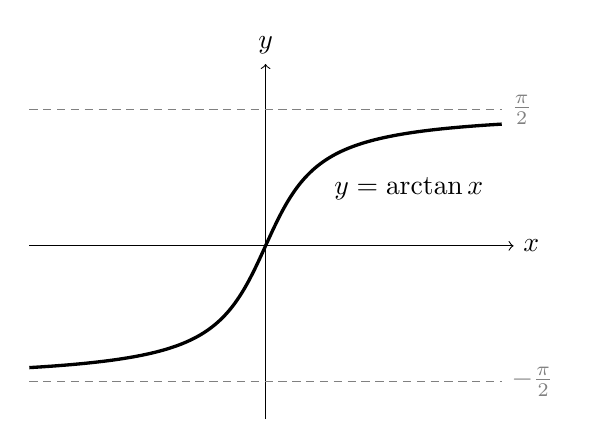
\begin{tikzpicture}[x=0.5cm, y=1.1cm]
    \draw[->] (-6,0) -- (6.3,0) node[right] {$x$};
    \draw[->] (0,-2) -- (0,2.1) node[above] {$y$};
    \draw[densely dashed, gray] (-6,1.5708) -- (6,1.5708)
      node[right] {$\frac\pi2$};
    \draw[densely dashed, gray] (-6,-1.5708) -- (6,-1.5708)
      node[right] {$-\frac\pi2$};
    \draw[very thick, domain=-6:6, samples=100, smooth]
      plot (\x, {rad(atan(\x))});
    \node[below right] at (1.5,0.9) {$y=\arctan x$};
  \end{tikzpicture}
\end{center}

\begin{theorem}
  $\arctan$ is differentiable on $\mathbb{R}$, and
  \[
    \frac{d}{dx}\arctan x=\frac{1}{1+x^2}.
  \]
\end{theorem}

\begin{proof}
  Apply Corollary~\ref{cor:inverse-derivative} to $f=\tan$ on
  $I=(-\frac\pi2,\frac\pi2)$, where $f'(\theta)=\sec^2\theta>0$; here
  $J=\mathbb{R}$. For any $x$, let $\theta=\arctan x$. Then
  \[
    \frac{d}{dx}\arctan x=\frac{1}{\sec^2\theta}
      =\frac{1}{1+\tan^2\theta}=\frac{1}{1+x^2}.
  \]
  (No sign issue arises this time.)
\end{proof}

\begin{example}
  $\dfrac{d}{dx}\arctan\sqrt{x}=\dfrac{1}{1+x}\cdot\dfrac{1}{2\sqrt{x}}
  =\dfrac{1}{2\sqrt{x}\,(1+x)}$, for $x>0$.
\end{example}

\begin{proposition}
  For $x>0$, $\arctan x+\arctan\dfrac1x=\dfrac\pi2$.
\end{proposition}

\begin{proof}
  Let $g(x)=\arctan x+\arctan(1/x)$ for $x>0$. Then
  \[
    g'(x)=\frac{1}{1+x^2}+\frac{1}{1+1/x^2}\cdot\Bigl(-\frac{1}{x^2}\Bigr)
      =\frac{1}{1+x^2}-\frac{1}{x^2+1}=0.
  \]
  A function with zero derivative on an interval is constant (by the MVT), so
  $g$ is constant on $(0,\infty)$, and $g(x)=g(1)=\frac\pi4+\frac\pi4
  =\frac\pi2$.
\end{proof}

\begin{remark}
  Geometrically: in a right triangle with legs $1$ and $x$, the two acute
  angles are $\arctan x$ and $\arctan(1/x)$.

  The same computation shows $g'(x)=0$ for $x<0$ too, but there
  $g(x)=-\frac\pi2$ (because $\arctan$ is odd). So $g$ has derivative $0$
  on all of $\mathbb{R}\setminus\{0\}$ without being constant. This does not
  contradict the MVT, because $\mathbb{R}\setminus\{0\}$ is not an interval.
\end{remark}

\subsection{Arcsecant}

On $[0,\pi]$, $\cos$ is strictly decreasing, so it is one-to-one. Removing
$\frac\pi2$, where $\cos$ is $0$, the function $\sec=1/\cos$ is one-to-one on
$[0,\frac\pi2)\cup(\frac\pi2,\pi]$. On $[0,\frac\pi2)$ it takes every value in
$[1,\infty)$, and on $(\frac\pi2,\pi]$ every value in $(-\infty,-1]$.

\begin{definition}
  For $|x|\geq1$, $\arcsec x$ is the unique number $\theta$ in
  $[0,\frac\pi2)\cup(\frac\pi2,\pi]$ with $\sec\theta=x$; equivalently, with
  $\cos\theta=\frac1x$.
\end{definition}

\begin{itemize}[itemsep=0.2em]
  \item The domain of $\arcsec$ is $(-\infty,-1]\cup[1,\infty)$, and its range
    is $[0,\frac\pi2)\cup(\frac\pi2,\pi]$.
  \item Values: $\arcsec1=0$, $\arcsec\sqrt2=\frac\pi4$,
    $\arcsec2=\frac\pi3$, $\arcsec(-2)=\frac{2\pi}{3}$,
    $\arcsec(-\sqrt2)=\frac{3\pi}{4}$, $\arcsec(-1)=\pi$.
  \item $\arcsec x\to\frac\pi2$ as $x\to\pm\infty$, since
    $\cos(\arcsec x)=\frac1x\to0$.
  \item $\arcsec$ is increasing on each of $[1,\infty)$ and $(-\infty,-1]$, but
    it is not increasing on its whole domain: $\arcsec(-2)>\arcsec2$.
\end{itemize}

\begin{center}
  \begin{tikzpicture}[x=0.5cm, y=1.1cm]
    \draw[->] (-6,0) -- (6.3,0) node[right] {$x$};
    \draw[->] (0,-0.4) -- (0,3.6) node[above] {$y$};
    \draw[densely dashed, gray] (-6,1.5708) -- (6,1.5708)
      node[right] {$\frac\pi2$};
    \draw[densely dotted, gray] (-6,3.1416) -- (6,3.1416)
      node[right] {$\pi$};
    % Parametrize by theta to get the vertical tangents at x = 1 and x = -1;
    % theta = acos(1/5) = 1.3694 gives x = 5.
    \draw[very thick, variable=\t, domain=0:1.3694, samples=60, smooth]
      plot ({1/cos(\t r)}, \t);
    \draw[very thick, variable=\t, domain=1.7722:3.1416, samples=60, smooth]
      plot ({1/cos(\t r)}, \t);
    \foreach \v in {-1,1} \draw (\v,0.05) -- (\v,-0.05) node[below] {$\v$};
    \node at (4.3,0.6) {$y=\arcsec x$};
  \end{tikzpicture}
\end{center}

\begin{theorem}
  $\arcsec$ is differentiable for $|x|>1$, and
  \[
    \frac{d}{dx}\arcsec x=\frac{1}{|x|\sqrt{x^2-1}}
    \qquad(|x|>1).
  \]
\end{theorem}

\begin{proof}
  We have $\sec'\theta=\sec\theta\tan\theta=\dfrac{\sin\theta}{\cos^2\theta}$,
  which is positive on $(0,\frac\pi2)$ and on $(\frac\pi2,\pi)$. Apply
  Corollary~\ref{cor:inverse-derivative} separately on $I_1=(0,\frac\pi2)$,
  where $J_1=(1,\infty)$, and on $I_2=(\frac\pi2,\pi)$, where
  $J_2=(-\infty,-1)$. For $|x|>1$, let $\theta=\arcsec x$. Then
  \[
    \frac{d}{dx}\arcsec x=\frac{1}{\sec\theta\tan\theta}
      =\frac{1}{x\tan\theta}.
  \]
  Now $\tan^2\theta=\sec^2\theta-1=x^2-1$, so
  $\tan\theta=\pm\sqrt{x^2-1}$, and we need the sign:
  \begin{itemize}[itemsep=0.2em]
    \item if $x>1$, then $\theta\in(0,\frac\pi2)$, so $\tan\theta>0$;
    \item if $x<-1$, then $\theta\in(\frac\pi2,\pi)$, so $\tan\theta<0$.
  \end{itemize}
  So $\tan\theta$ has the same sign as $x$, and
  $x\tan\theta=|x|\sqrt{x^2-1}$.
\end{proof}

\begin{example}
  $\dfrac{d}{dx}\arcsec(x^2)=\dfrac{2x}{x^2\sqrt{x^4-1}}
  =\dfrac{2}{x\sqrt{x^4-1}}$, for $|x|>1$. (Here $|x^2|=x^2$.)
\end{example}

\begin{remark}
  Some textbooks restrict $\sec$ to $[0,\frac\pi2)\cup[\pi,\frac{3\pi}{2})$
  instead. With that convention, $\frac{d}{dx}\arcsec x=\frac{1}{x\sqrt{x^2-1}}$
  with no absolute value, but values such as $\arcsec(-2)$ change. Students
  who look at other references may run into this.
\end{remark}

\subsection{The other three}

\begin{itemize}[itemsep=0.4em]
  \item $\arccos x$, for $-1\leq x\leq1$, is the unique $\theta\in[0,\pi]$
    with $\cos\theta=x$. Since $\theta=\frac\pi2-\arcsin x$ lies in $[0,\pi]$
    and $\cos\bigl(\frac\pi2-\arcsin x\bigr)=\sin(\arcsin x)=x$,
    \[
      \arccos x=\frac\pi2-\arcsin x,
      \qquad
      \frac{d}{dx}\arccos x=-\frac{1}{\sqrt{1-x^2}}.
    \]
  \item $\arccot x$, for all real $x$, is the unique $\theta\in(0,\pi)$ with
    $\cot\theta=x$. In the same way,
    \[
      \arccot x=\frac\pi2-\arctan x,
      \qquad
      \frac{d}{dx}\arccot x=-\frac{1}{1+x^2}.
    \]
  \item $\arccsc x$, for $|x|\geq1$, is the unique
    $\theta\in[-\frac\pi2,0)\cup(0,\frac\pi2]$ with $\csc\theta=x$. Again,
    \[
      \arccsc x=\frac\pi2-\arcsec x,
      \qquad
      \frac{d}{dx}\arccsc x=-\frac{1}{|x|\sqrt{x^2-1}}.
    \]
\end{itemize}

For integration these give nothing new, since each derivative is the negative
of one we already have.

\subsection{Summary}

\begin{center}
  \renewcommand{\arraystretch}{2.1}
  \begin{tabular}{|c|c|c|c|}
    \hline
    \textbf{Function} & \textbf{Domain} & \textbf{Range}
      & \textbf{Derivative} \\
    \hline
    $\arcsin x$ & $[-1,1]$ & $[-\frac\pi2,\frac\pi2]$
      & $\dfrac{1}{\sqrt{1-x^2}}$\quad$(|x|<1)$ \\
    \hline
    $\arctan x$ & $\mathbb{R}$ & $(-\frac\pi2,\frac\pi2)$
      & $\dfrac{1}{1+x^2}$ \\
    \hline
    $\arcsec x$ & $|x|\geq1$ & $[0,\frac\pi2)\cup(\frac\pi2,\pi]$
      & $\dfrac{1}{|x|\sqrt{x^2-1}}$\quad$(|x|>1)$ \\
    \hline
    $\arccos x$ & $[-1,1]$ & $[0,\pi]$
      & $-\dfrac{1}{\sqrt{1-x^2}}$\quad$(|x|<1)$ \\
    \hline
    $\arccot x$ & $\mathbb{R}$ & $(0,\pi)$
      & $-\dfrac{1}{1+x^2}$ \\
    \hline
    $\arccsc x$ & $|x|\geq1$ & $[-\frac\pi2,0)\cup(0,\frac\pi2]$
      & $-\dfrac{1}{|x|\sqrt{x^2-1}}$\quad$(|x|>1)$ \\
    \hline
  \end{tabular}
\end{center}

\subsection{Simplifying compositions}\label{sec:triangles}

Expressions like $\tan(\arcsin x)$ can be rewritten without trigonometric
functions. The method: name the angle, use a Pythagorean identity, and use the
range of the inverse function to fix the sign. A right triangle (drawn for
$x>0$) shows what the answer should be.

\begin{center}
  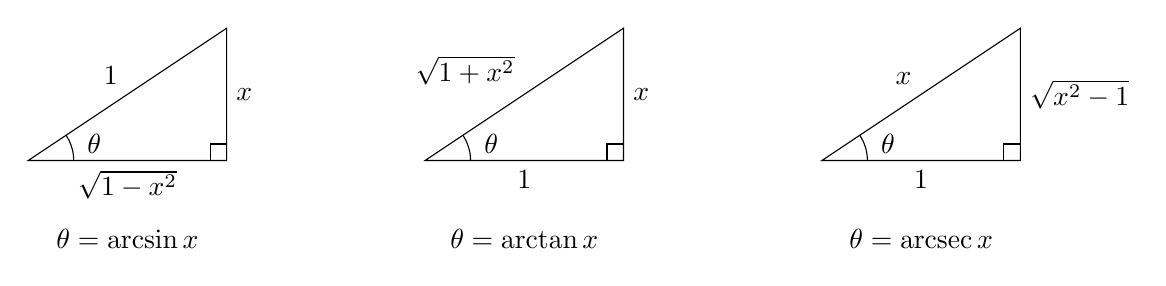
\begin{tikzpicture}[scale=1.05]
    \begin{scope}
      \draw (0,0) -- (2.4,0) -- (2.4,1.6) -- cycle;
      \draw (2.2,0) -- (2.2,0.2) -- (2.4,0.2);
      \draw (0.55,0) arc[start angle=0, end angle={atan(1.6/2.4)},
        radius=0.55];
      \node at (0.8,0.2) {$\theta$};
      \node[below] at (1.2,0) {$\sqrt{1-x^2}$};
      \node[right] at (2.4,0.8) {$x$};
      \node[above left] at (1.2,0.8) {$1$};
      \node at (1.2,-0.95) {$\theta=\arcsin x$};
    \end{scope}
    \begin{scope}[xshift=4.8cm]
      \draw (0,0) -- (2.4,0) -- (2.4,1.6) -- cycle;
      \draw (2.2,0) -- (2.2,0.2) -- (2.4,0.2);
      \draw (0.55,0) arc[start angle=0, end angle={atan(1.6/2.4)},
        radius=0.55];
      \node at (0.8,0.2) {$\theta$};
      \node[below] at (1.2,0) {$1$};
      \node[right] at (2.4,0.8) {$x$};
      \node[above left] at (1.2,0.8) {$\sqrt{1+x^2}$};
      \node at (1.2,-0.95) {$\theta=\arctan x$};
    \end{scope}
    \begin{scope}[xshift=9.6cm]
      \draw (0,0) -- (2.4,0) -- (2.4,1.6) -- cycle;
      \draw (2.2,0) -- (2.2,0.2) -- (2.4,0.2);
      \draw (0.55,0) arc[start angle=0, end angle={atan(1.6/2.4)},
        radius=0.55];
      \node at (0.8,0.2) {$\theta$};
      \node[below] at (1.2,0) {$1$};
      \node[right] at (2.4,0.8) {$\sqrt{x^2-1}$};
      \node[above left] at (1.2,0.8) {$x$};
      \node at (1.2,-0.95) {$\theta=\arcsec x$};
    \end{scope}
  \end{tikzpicture}
\end{center}

\begin{example}
  Simplify $\tan(\arcsin x)$ for $-1<x<1$.

  Let $\theta=\arcsin x$, so $\sin\theta=x$. Since
  $\theta\in[-\frac\pi2,\frac\pi2]$, $\cos\theta\geq0$, so
  $\cos\theta=\sqrt{1-x^2}$. Therefore
  $\tan(\arcsin x)=\dfrac{x}{\sqrt{1-x^2}}$.
\end{example}

\begin{example}
  Simplify $\cos(\arctan x)$ and $\sin(\arctan x)$.

  Let $\theta=\arctan x\in(-\frac\pi2,\frac\pi2)$. Then $\cos\theta>0$ and
  $\sec^2\theta=1+\tan^2\theta=1+x^2$, so
  \[
    \cos(\arctan x)=\frac{1}{\sqrt{1+x^2}},\qquad
    \sin(\arctan x)=\tan\theta\cos\theta=\frac{x}{\sqrt{1+x^2}}.
  \]
  For instance, $\sin(2\arctan x)=2\sin\theta\cos\theta=\dfrac{2x}{1+x^2}$.
\end{example}

\begin{example}
  Find $\sin\bigl(\arcsec(-3)\bigr)$.

  Let $\theta=\arcsec(-3)$, so $\cos\theta=-\frac13$ and
  $\theta\in(\frac\pi2,\pi)$. There $\sin\theta>0$, so
  $\sin\theta=\sqrt{1-\frac19}=\frac{2\sqrt2}{3}$. (The triangle alone would
  not tell us the sign.)
\end{example}

When we get to trigonometric substitution, we will use these same triangles
in reverse.

\subsection{Integrals}

Reading the derivative formulas backwards gives
\[
  \boxed{\;
  \begin{aligned}
    \int\frac{dx}{\sqrt{1-x^2}}&=\arcsin x+C,\\
    \int\frac{dx}{1+x^2}&=\arctan x+C,\\
    \int\frac{dx}{x\sqrt{x^2-1}}&=\arcsec|x|+C.
  \end{aligned}
  \;}
\]
The third formula needs a comment. For $x>1$ it is the derivative formula,
since $|x|=x$. For $x<-1$,
\[
  \frac{d}{dx}\arcsec|x|=\frac{d}{dx}\arcsec(-x)
    =-\frac{1}{|x|\sqrt{x^2-1}}=\frac{1}{x\sqrt{x^2-1}},
\]
since $-|x|=x$ when $x<0$. Compare $\int\frac{dx}{x}=\ln|x|+C$.

More generally, for a constant $a>0$,
\[
  \boxed{\;
  \begin{aligned}
    \int\frac{dx}{\sqrt{a^2-x^2}}&=\arcsin\frac{x}{a}+C,\\
    \int\frac{dx}{a^2+x^2}&=\frac1a\arctan\frac{x}{a}+C,\\
    \int\frac{dx}{x\sqrt{x^2-a^2}}&=\frac1a\arcsec\frac{|x|}{a}+C.
  \end{aligned}
  \;}
\]
These follow from the first three by the substitution $u=x/a$. For example,
with $x=au$ and $dx=a\,du$,
\[
  \int\frac{dx}{a^2+x^2}=\int\frac{a\,du}{a^2(1+u^2)}
    =\frac1a\arctan u+C=\frac1a\arctan\frac xa+C.
\]
Rather than memorizing the general versions, one can always substitute.

\begin{example}
  \begin{enumerate}[label=(\alph*)]
    \item $\displaystyle\int_0^1\frac{dx}{1+x^2}=\arctan1-\arctan0
      =\frac\pi4$.
      (So Riemann sums for $\frac{4}{1+x^2}$ on $[0,1]$ approximate $\pi$.)
    \item $\displaystyle\int_0^{1/2}\frac{dx}{\sqrt{1-x^2}}
      =\arcsin\frac12-\arcsin0=\frac\pi6$.
  \end{enumerate}
\end{example}

\begin{example}
  $\displaystyle\int\frac{dx}{\sqrt{4-9x^2}}$. Let $u=3x$, so $du=3\,dx$:
  \[
    \int\frac{dx}{\sqrt{4-9x^2}}=\frac13\int\frac{du}{\sqrt{4-u^2}}
      =\frac13\arcsin\frac u2+C=\frac13\arcsin\frac{3x}{2}+C.
  \]
\end{example}

\begin{example}
  Compare $\displaystyle\int\frac{dx}{1+x^2}=\arctan x+C$ with
  $\displaystyle\int\frac{x\,dx}{1+x^2}$, where $u=1+x^2$ gives
  $\frac12\ln(1+x^2)+C$. Similar-looking integrands can have very different
  antiderivatives. Splitting a fraction uses both:
  \[
    \int\frac{x+3}{1+x^2}\,dx=\int\frac{x}{1+x^2}\,dx+3\int\frac{dx}{1+x^2}
      =\frac12\ln(1+x^2)+3\arctan x+C.
  \]
\end{example}

\begin{example}
  $\displaystyle\int\frac{x}{1+x^4}\,dx$. Let $u=x^2$, so $du=2x\,dx$:
  \[
    \int\frac{x}{1+x^4}\,dx=\frac12\int\frac{du}{1+u^2}
      =\frac12\arctan u+C=\frac12\arctan(x^2)+C.
  \]
\end{example}

\begin{example}[Completing the square]
  \begin{enumerate}[label=(\alph*)]
    \item $\displaystyle\int\frac{dx}{x^2+4x+13}$. Since
      $x^2+4x+13=(x+2)^2+9$, let $u=x+2$:
      \[
        \int\frac{dx}{(x+2)^2+9}=\int\frac{du}{u^2+9}
          =\frac13\arctan\frac u3+C=\frac13\arctan\frac{x+2}{3}+C.
      \]
    \item $\displaystyle\int\frac{dx}{\sqrt{6x-x^2}}$. Since
      $6x-x^2=9-(x-3)^2$, let $u=x-3$:
      \[
        \int\frac{dx}{\sqrt{9-(x-3)^2}}=\int\frac{du}{\sqrt{9-u^2}}
          =\arcsin\frac u3+C=\arcsin\frac{x-3}{3}+C.
      \]
  \end{enumerate}
\end{example}

\begin{example}
  $\displaystyle\int\frac{e^x}{\sqrt{1-e^{2x}}}\,dx$. Let $u=e^x$, so
  $du=e^x\,dx$:
  \[
    \int\frac{e^x}{\sqrt{1-e^{2x}}}\,dx=\int\frac{du}{\sqrt{1-u^2}}
      =\arcsin(e^x)+C.
  \]
\end{example}

\begin{example}
  \begin{enumerate}[label=(\alph*)]
    \item $\displaystyle\int_{\sqrt2}^{2}\frac{dx}{x\sqrt{x^2-1}}
      =\arcsec2-\arcsec\sqrt2=\frac\pi3-\frac\pi4=\frac{\pi}{12}$.
    \item $\displaystyle\int_{-2}^{-\sqrt2}\frac{dx}{x\sqrt{x^2-1}}
      =\Bigl[\arcsec|x|\Bigr]_{-2}^{-\sqrt2}
      =\arcsec\sqrt2-\arcsec2=-\frac{\pi}{12}$.
      This should be negative, since the integrand is negative for $x<0$.
      Dropping the absolute value would give
      $\arcsec(-\sqrt2)-\arcsec(-2)=\frac{3\pi}{4}-\frac{2\pi}{3}
      =\frac{\pi}{12}$, which has the wrong sign.
  \end{enumerate}
\end{example}

\begin{example}
  For $b>0$, the area under $y=\frac{1}{1+x^2}$ from $0$ to $b$ is
  \[
    A(b)=\int_0^b\frac{dx}{1+x^2}=\arctan b,
  \]
  and $A(b)\to\frac\pi2$ as $b\to\infty$. So although the region under the
  whole curve is infinitely long, the area of the part with $0\leq x\leq b$
  never exceeds $\frac\pi2$. By symmetry, the same holds on the left, for a
  total of $\pi$.
\end{example}

%----------------------------------------------------------------------------
\section{Integration by parts}\label{sec:parts}

Substitution is the chain rule run backwards; integration by parts is the
product rule run backwards.

\begin{theorem}[Integration by parts]
  Suppose $u$ and $v$ have continuous derivatives on an interval. Then
  \[
    \int u(x)\,v'(x)\,dx=u(x)\,v(x)-\int v(x)\,u'(x)\,dx,
  \]
  and for $a$ and $b$ in the interval,
  \[
    \int_a^b u(x)\,v'(x)\,dx=\Bigl[u(x)\,v(x)\Bigr]_a^b
      -\int_a^b v(x)\,u'(x)\,dx.
  \]
\end{theorem}

\begin{proof}
  By the product rule, the derivative of the right side of the first formula
  is $(u'v+uv')-vu'=uv'$, so the right side is an antiderivative of $uv'$.
  For the second formula, integrate $(uv)'=u'v+uv'$ from $a$ to $b$. By the
  Fundamental Theorem of Calculus, $\int_a^b(uv)'\,dx=\bigl[uv\bigr]_a^b$.
  (All the integrands are continuous, so all the integrals exist.)
\end{proof}

\textbf{Shorthand.} With $du=u'(x)\,dx$ and $dv=v'(x)\,dx$, the formula reads
\[
  \boxed{\;\int u\,dv=uv-\int v\,du.\;}
\]

\textbf{How to choose.} Write the integrand as $u\cdot dv$, where
\begin{itemize}[itemsep=0.2em]
  \item you can integrate $dv$ to find $v$, and
  \item $\int v\,du$ is simpler than the original integral.
\end{itemize}
Rule of thumb: take $u$ to be something that becomes simpler when
differentiated (a polynomial, $\ln x$, an inverse trigonometric function), and
$dv$ to be something that does not become worse when integrated ($e^x$,
$\sin x$, $\cos x$, or just $dx$).

Any antiderivative $v$ works, so we always take the simplest one, with
constant $0$. (Replacing $v$ by $v+c$ adds $cu$ to $uv$ and $cu$ to
$\int v\,du$, and these cancel.)

\begin{example}
  $\displaystyle\int xe^x\,dx$. Let $u=x$ and $dv=e^x\,dx$, so $du=dx$ and
  $v=e^x$:
  \[
    \int xe^x\,dx=xe^x-\int e^x\,dx=xe^x-e^x+C.
  \]
  Check: $\frac{d}{dx}(xe^x-e^x)=e^x+xe^x-e^x=xe^x$.

  \emph{A bad choice:} $u=e^x$ and $dv=x\,dx$ give $du=e^x\,dx$ and
  $v=\frac{x^2}{2}$, so
  \[
    \int xe^x\,dx=\frac{x^2}{2}e^x-\int\frac{x^2}{2}e^x\,dx,
  \]
  which is correct but leaves a harder integral than the one we started with.
\end{example}

\begin{example}
  $\displaystyle\int_0^\pi x\sin x\,dx$. Let $u=x$ and $dv=\sin x\,dx$, so
  $du=dx$ and $v=-\cos x$:
  \[
    \int_0^\pi x\sin x\,dx=\Bigl[-x\cos x\Bigr]_0^\pi+\int_0^\pi\cos x\,dx
      =\pi+\Bigl[\sin x\Bigr]_0^\pi=\pi.
  \]
\end{example}

\begin{example}
  $\displaystyle\int\ln x\,dx$. There is no visible product, but we can take
  $u=\ln x$ and $dv=dx$, so $du=\frac{dx}{x}$ and $v=x$:
  \[
    \int\ln x\,dx=x\ln x-\int x\cdot\frac1x\,dx=x\ln x-x+C.
  \]
\end{example}

\begin{example}
  $\displaystyle\int x\ln x\,dx$. Here the rule of thumb says to take
  $u=\ln x$, even though $x$ is a polynomial: we can't easily integrate
  $\ln x$, but differentiating it makes it simpler. With $u=\ln x$ and
  $dv=x\,dx$, we have $du=\frac{dx}{x}$ and $v=\frac{x^2}{2}$, so
  \[
    \int x\ln x\,dx=\frac{x^2}{2}\ln x-\int\frac{x^2}{2}\cdot\frac1x\,dx
      =\frac{x^2}{2}\ln x-\frac{x^2}{4}+C.
  \]
\end{example}

\begin{example}[Inverse trigonometric functions]
  \begin{enumerate}[label=(\alph*)]
    \item $\displaystyle\int\arctan x\,dx$. Let $u=\arctan x$ and $dv=dx$, so
      $du=\frac{dx}{1+x^2}$ and $v=x$:
      \[
        \int\arctan x\,dx=x\arctan x-\int\frac{x}{1+x^2}\,dx
          =x\arctan x-\frac12\ln(1+x^2)+C.
      \]
    \item $\displaystyle\int\arcsin x\,dx$. Let $u=\arcsin x$ and $dv=dx$, so
      $du=\frac{dx}{\sqrt{1-x^2}}$ and $v=x$:
      \[
        \int\arcsin x\,dx=x\arcsin x-\int\frac{x}{\sqrt{1-x^2}}\,dx.
      \]
      For the last integral, let $w=1-x^2$, so $dw=-2x\,dx$:
      $\int\frac{x\,dx}{\sqrt{1-x^2}}=-\frac12\int w^{-1/2}\,dw
      =-\sqrt{1-x^2}+C$. So
      \[
        \int\arcsin x\,dx=x\arcsin x+\sqrt{1-x^2}+C,
      \]
      which agrees with what we checked in Section~\ref{sec:inverse-trig}.
  \end{enumerate}
\end{example}

\begin{example}[Integrating by parts twice]
  $\displaystyle\int x^2e^x\,dx$. Let $u=x^2$ and $dv=e^x\,dx$, so
  $du=2x\,dx$ and $v=e^x$:
  \[
    \int x^2e^x\,dx=x^2e^x-2\int xe^x\,dx=x^2e^x-2(xe^x-e^x)+C
      =(x^2-2x+2)e^x+C,
  \]
  using the earlier example for $\int xe^x\,dx$.

  The same choice for $\int x^ne^x\,dx$ gives the \emph{reduction formula}
  \[
    \int x^ne^x\,dx=x^ne^x-n\int x^{n-1}e^x\,dx,
  \]
  which lowers the power of $x$ by one each time. For example,
  \[
    \int x^3e^x\,dx=x^3e^x-3\int x^2e^x\,dx=(x^3-3x^2+6x-6)e^x+C.
  \]
\end{example}

\begin{example}[Solving for the integral]
  $\displaystyle I=\int e^x\sin x\,dx$. Let $u=e^x$ and $dv=\sin x\,dx$, so
  $du=e^x\,dx$ and $v=-\cos x$:
  \[
    I=-e^x\cos x+\int e^x\cos x\,dx.
  \]
  Integrate by parts again with $u=e^x$ and $dv=\cos x\,dx$, so $v=\sin x$:
  \[
    \int e^x\cos x\,dx=e^x\sin x-\int e^x\sin x\,dx=e^x\sin x-I.
  \]
  So $I=-e^x\cos x+e^x\sin x-I$, and solving for $I$,
  \[
    \int e^x\sin x\,dx=\frac12e^x(\sin x-\cos x)+C.
  \]
  Check: $\frac{d}{dx}\bigl[\frac12e^x(\sin x-\cos x)\bigr]
  =\frac12e^x(\sin x-\cos x)+\frac12e^x(\cos x+\sin x)=e^x\sin x$.

  \emph{Warning:} in the second step we must again take $u=e^x$. Choosing
  $u=\cos x$ and $dv=e^x\,dx$ instead just undoes the first step and leads to
  $I=I$.
\end{example}

\begin{example}[Substitution and parts together]
  $\displaystyle\int x^3e^{x^2}\,dx$. Write the integrand as
  $x^2\cdot xe^{x^2}$, and let $u=x^2$ and $dv=xe^{x^2}\,dx$. Then
  $du=2x\,dx$ and, by the substitution $w=x^2$, $v=\frac12e^{x^2}$. So
  \[
    \int x^3e^{x^2}\,dx=\frac12x^2e^{x^2}-\int xe^{x^2}\,dx
      =\frac12x^2e^{x^2}-\frac12e^{x^2}+C
      =\frac12(x^2-1)e^{x^2}+C.
  \]
  (Alternatively, substitute $w=x^2$ first to get
  $\frac12\int we^w\,dw$, and then integrate by parts.)
\end{example}

\begin{example}[A volume]
  The region under $y=\cos x$ for $0\leq x\leq\frac\pi2$ is revolved about
  the $y$-axis. By the shell method, the volume is
  \[
    V=\int_0^{\pi/2}2\pi x\cos x\,dx.
  \]
  Let $u=x$ and $dv=\cos x\,dx$, so $du=dx$ and $v=\sin x$:
  \[
    \int_0^{\pi/2}x\cos x\,dx=\Bigl[x\sin x\Bigr]_0^{\pi/2}
      -\int_0^{\pi/2}\sin x\,dx
      =\frac\pi2-\Bigl[-\cos x\Bigr]_0^{\pi/2}=\frac\pi2-1.
  \]
  So $V=2\pi\bigl(\frac\pi2-1\bigr)=\pi^2-2\pi$.
\end{example}

\textbf{Optional: integrating an inverse function.} The integrals of
$\ln x$, $\arctan x$, and $\arcsin x$ above all have the same shape, and the
reason ties together everything in these notes.

\begin{proposition}
  Let $f$ be differentiable with $f'>0$ (or $f'<0$) on an open interval, and
  let $F$ be an antiderivative of $f$. Then
  \[
    \int f^{-1}(x)\,dx=x\,f^{-1}(x)-F\bigl(f^{-1}(x)\bigr)+C.
  \]
\end{proposition}

\begin{proof}
  By Corollary~\ref{cor:inverse-derivative}, $f^{-1}$ is differentiable, so
  we can differentiate the right side:
  \[
    f^{-1}(x)+x\,(f^{-1})'(x)-f\bigl(f^{-1}(x)\bigr)\,(f^{-1})'(x)
      =f^{-1}(x),
  \]
  since $f\bigl(f^{-1}(x)\bigr)=x$.
\end{proof}

This is what integration by parts with $u=f^{-1}(x)$ and $dv=dx$ produces,
followed by the substitution $y=f^{-1}(x)$ in $\int x\,(f^{-1})'(x)\,dx$.
Examples:
\begin{itemize}[itemsep=0.2em]
  \item $f=\exp$, $F=\exp$:\quad
    $\int\ln x\,dx=x\ln x-e^{\ln x}+C=x\ln x-x+C$.
  \item $f=\sin$, $F=-\cos$:\quad
    $\int\arcsin x\,dx=x\arcsin x+\cos(\arcsin x)+C
    =x\arcsin x+\sqrt{1-x^2}+C$.
  \item $f=\tan$, $F(y)=\ln|\sec y|$:\quad
    $\int\arctan x\,dx=x\arctan x-\ln\bigl|\sec(\arctan x)\bigr|+C
    =x\arctan x-\frac12\ln(1+x^2)+C$,
    since $\sec(\arctan x)=\sqrt{1+x^2}$.
\end{itemize}

\end{document}
